\documentclass[11pt,a4paper]{article}

\usepackage{blockdiagram}
\usepackage{verbatim}
\usepackage{amsmath}

\title{The \textbf{blockdiagram} package}

\author{Guillaume J. Laurent}

\date{July 25, 2009}

\begin{document}
\maketitle

The \textbf{blockdiagram} package is a set of tikz macros to draw nice block diagrams.

\section{Transfer function}

\footnotesize
\begin{verbatim}
\begin{tikzpicture}
  \inputnode{I}
  \blockr{I}{G}{$\frac{K}{1+\tau s}$}
  \link{I}{G}{$u$}
  \outputnode{G}{O}
  \link{G}{O}{$y$}
\end{tikzpicture} 
\end{verbatim}

\begin{center}
\begin{tikzpicture}[scale=2]
	\inputnode{I}
	\blockr{I}{G}{$\dfrac{K}{1+\tau s}$}
	\link{I}{G}{$u$}
	\outputnode{G}{O}
	\link{G}{O}{$y$}
\end{tikzpicture} 
\end{center}

\section{Feedback Loop}

\footnotesize
\begin{verbatim}
\begin{tikzpicture}
  \inputnode{I}
  \sumblockr{I}{S}{}{+}{-}{}
  \link{I}{S}{$r$}
  \blockr{S}{C}{Controller}
  \link{S}{C}{$e$}
  \blockr[3cm]{C}{P}{Plant}
  \link{C}{P}{$u$}
  \outputnode{P}{O}
  \link{P}{O}{$y$}
  \yxylink{P-O}{S}{$y$}
\end{tikzpicture} 
\end{verbatim}

\begin{center}
\begin{tikzpicture}
	\inputnode{I}
	\sumblockr{I}{S}{}{+}{-}{}
	\link{I}{S}{$r$}
	\blockr{S}{C}{Controller}
	\link{S}{C}{$e$}
	\blockr[3cm]{C}{P}{Plant}
	\link{C}{P}{$u$}
	\outputnode{P}{O}
	\link{P}{O}{$y$}
	\yxylink{P-O}{S}{$y$}
\end{tikzpicture} 
\end{center}

\newpage

\section{Another Feedback Loop}

\footnotesize
\begin{verbatim}
\begin{tikzpicture}
  \inputnode{I}
  \sumblockr{I}{S}{}{+}{-}{}
  \link{I}{S}{$r$}
  \blockr{S}{C}{Controller}
  \link{S}{C}{$e$}
  \plantblockr[3cm]{C}{P}{Plant}
  \link{C}{P}{$u$}
  \nodea{P}{D}
  \ylink{D}{P}{Disturbances}
  \outputnode{P}{O}
  \link{P}{O}{$y$}
  \blockb{C-P}{M}{Measurement}
  \yxlink{P-O}{M}{}
  \xylink{M}{S}{$y_m$}
\end{tikzpicture} 
\end{verbatim}

\begin{center}
\begin{tikzpicture}
	\inputnode{I}
	\sumblockr{I}{S}{}{+}{-}{}
	\link{I}{S}{$r$}
	\blockr{S}{C}{Controller}
	\link{S}{C}{$e$}
	\plantblockr[3cm]{C}{P}{Plant}
	\link{C}{P}{$u$}
	\nodea{P}{D}
	\ylink{D}{P}{Disturbances}
	\outputnode{P}{O}
	\link{P}{O}{$y$}
	\blockb{C-P}{M}{Measurement}
	\yxlink{P-O}{M}{}
	\xylink{M}{S}{$y_m$}
\end{tikzpicture} 
\end{center}

\section{Linear Quadratic Regulator}

\footnotesize
\begin{verbatim}
\begin{tikzpicture}\setdiagramscale{0.8}
  \inputnode{E}
  \blockr{E}{filter}{$S$}
  \link{E}{filter}{$r$}
  \sumblockr{filter}{sum2}{}{+}{-}{}
  \link{filter}{sum2}{}
  \blockr{sum2}{command}{$B$}
  \link{sum2}{command}{$u$}
  \sumblockr{command}{sum1}{}{+}{+}{}
  \link{command}{sum1}{}
  \blockr{sum1}{integrator}{$\int$}
  \link{sum1}{integrator}{$\dot{X}$}
  \blockr[3cm]{integrator}{obs}{$C$}
  \link{integrator}{obs}{$X$}
  \outputnode{obs}{S}
  \link{obs}{S}{$y$}
  \blockb{integrator}{evolution}{$A$}
  \yxlink{integrator-obs}{evolution}{}
  \xylink{evolution}{sum1}{}
  \blockb{evolution}{regulator}{$L$}
  \yxlink{integrator-obs}{regulator}{}
  \xylink{regulator}{sum2}{}
\end{tikzpicture}
\end{verbatim}

\begin{center}
\begin{tikzpicture}\setdiagramscale{0.8}
  \inputnode{E}
  \blockr{E}{filter}{$S$}
  \link{E}{filter}{$r$}
  \sumblockr{filter}{sum2}{}{+}{-}{}
  \link{filter}{sum2}{}
  \blockr{sum2}{command}{$B$}
  \link{sum2}{command}{$u$}
  \sumblockr{command}{sum1}{}{+}{+}{}
  \link{command}{sum1}{}
  \blockr{sum1}{integrator}{$\int$}
  \link{sum1}{integrator}{$\dot{X}$}
  \blockr[3cm]{integrator}{obs}{$C$}
  \link{integrator}{obs}{$X$}
  \outputnode{obs}{S}
  \link{obs}{S}{$y$}
  \blockb{integrator}{evolution}{$A$}
  \yxlink{integrator-obs}{evolution}{}
  \xylink{evolution}{sum1}{}
  \blockb{evolution}{regulator}{$L$}
  \yxlink{integrator-obs}{regulator}{}
  \xylink{regulator}{sum2}{}
\end{tikzpicture}
\end{center}

\section{Observator}

\footnotesize
\begin{verbatim}
\begin{tikzpicture}
  \inputnode{E}
  \plantblockr{E}{system}{Plant}
  \outputnode{system}{S}
  \link{E}{system}{$u$}
  \link{system}{S}{$y$}
  \noder[1cm]{S}{SS}
  \blockb{SS}{observator}{Observator}
  \yxlink{system-S}{observator.170}{}
  \yxlink{E-system}{observator.190}{}
  \noder{observator}{X}
  \link{observator}{X}{$\hat{X}$}
\end{tikzpicture}
\end{verbatim}

\begin{center}
\begin{tikzpicture}
	\inputnode{E}
	\plantblockr{E}{system}{Plant}
	\outputnode{system}{S}
	\link{E}{system}{$u$}
	\link{system}{S}{$y$}
	\noder[1cm]{S}{SS}
	\blockb{SS}{observator}{Observator}
	\yxlink{system-S}{observator.170}{}
	\yxlink{E-system}{observator.190}{}
	\noder{observator}{X}
	\link{observator}{X}{$\hat{X}$}
\end{tikzpicture}
\end{center}

\end{document}